\documentclass[11pt]{article}

\usepackage{amsmath}
\usepackage{amssymb}
\usepackage{graphicx}
\usepackage{booktabs}
\usepackage{geometry}
\usepackage{hyperref}
\usepackage{multirow}
\usepackage{subcaption}

\geometry{margin=1in}
\graphicspath{{figures/}}

\title{Which Exogenous Features Improve 1D-CNN Soil-Moisture\\
Forecasting? Evidence from the TxSON Network}
\author{Abijith Chandrasekar Vijayan}
\date{\today}

\begin{document}

\maketitle

\begin{abstract}
We study hourly soil-moisture forecasting at 20\,cm depth (\texttt{SWC\_20})
with a one-dimensional convolutional neural network (1D~CNN) on in-situ data
from the Texas Soil Observation Network (TxSON). The central question is which
\emph{exogenous} predictors---precipitation and its lagged/cumulative forms, air
temperature, humidity, and seasonality---most improve forecasts beyond
historical soil moisture alone. Using a shared CNN and a held-out station-year
protocol across four stations (FD11, FD02, CB06, CB25), five forecast horizons
(24--168\,h), and six feature configurations, we run 150 CNN experiments plus
25 persistence baselines, all evaluated in physical units with
training-only normalization and strictly causal features. We find that
\textbf{no exogenous feature consistently improves RMSE over a soil-moisture-only
model}: every configuration has a negative mean change and helps in at most
10 of 25 station-year$\times$horizon cells. Among exogenous inputs, air
temperature and single-step rainfall are the least harmful on average, while
stacking many features is the most harmful, especially at short horizons; the
one clear benefit is cumulative rainfall at the driest station (FD02, up to
$+13.4\%$). A separate lag analysis shows rainfall correlates with soil-moisture
change at a 1--2\,hour lag and, at the driest station, couples more tightly to
5\,cm than 20\,cm moisture---yet these correlations do not translate into lower
CNN forecast error. Results are single-seed and the architectural gains
($\sim$5\% from a deeper/wider CNN) rest on one station-year, so we frame the
findings as evidence that historical soil moisture dominates at these horizons
rather than as a definitive feature ranking.
\end{abstract}

% ============================================================================
\section{Introduction}
% ============================================================================

Soil moisture is a key variable in hydrology, agriculture, and climate science.
Accurate forecasts of near-surface soil water content inform irrigation
scheduling, drought monitoring, and land--atmosphere modeling. Because soil
moisture evolves over time---driven by precipitation, evapotranspiration, and
drainage---temporal forecasting is a natural framing: given a recent history of
observations, predict soil moisture some hours into the future.

Deep learning has been applied to this problem for its ability to learn
nonlinear temporal patterns directly from data \cite{liu2022multiscale}. Among
such models, 1D~CNNs are attractive for time-series forecasting
\cite{borovykh2017conditional, bai2018empirical}: the same learned filters are
applied across the input window, so a local event such as a rain-driven moisture
rise is detected regardless of where it occurs in the window.

For a time-series target, the strongest predictor is almost always the target's
own recent history. The scientific interest here is therefore not whether the
model works, but \textbf{which \emph{external} variables add predictive value on
top of historical soil moisture}. This report answers that question directly,
using hourly in-situ TxSON observations and a shared CNN evaluated across four
stations and five forecast horizons. We progress through: (1)~a precipitation
lag analysis establishing the physical rainfall$\rightarrow$moisture timescale;
(2)~a controlled multi-station feature comparison that ranks exogenous feature
groups by their effect on test RMSE; (3)~a small CNN hyperparameter sweep; and
(4)~training diagnostics for overfitting. An earlier single-station study and a
12-class classification formulation are summarized as complementary context.

% ============================================================================
\section{Related Work}
% ============================================================================

1D~CNNs and temporal convolutional networks have been shown to match or exceed
recurrent models on many sequence-modeling benchmarks \cite{bai2018empirical},
and convolutional architectures have been applied specifically to conditional
time-series forecasting \cite{borovykh2017conditional}. The convolutional
building blocks trace back to gradient-based learning for pattern recognition
\cite{lecun1998gradient}. For soil moisture specifically, deep models that
integrate satellite and in-situ measurements have been proposed
\cite{liu2022multiscale}. Our contribution is narrow and empirical: a controlled,
leakage-audited comparison of exogenous feature groups for CNN soil-moisture
forecasting on a single well-characterized in-situ network, with an explicit
focus on whether external predictors help rather than on absolute accuracy.

% ============================================================================
\section{Dataset and Preprocessing}
% ============================================================================

\subsection{Data Source and Stations}

We use the TxSON33 modeling-complete dataset: hourly measurements at 33 TxSON
stations (2{,}720{,}775 rows). Each record carries soil water content at 5, 10,
20, and 50\,cm (\texttt{SWC\_5/10/20/50}), soil temperature at the same depths
(\texttt{T\_5/\dots/T\_50}), air temperature (\texttt{Tair}), relative humidity
(\texttt{RH}), solar radiation (\texttt{Srad}), wind speed and direction, and
precipitation (\texttt{Ppt}). Companion \texttt{*\_Origin} columns record whether
each value is \texttt{observed}, \texttt{pipeline\_imputed}, or
\texttt{modeling\_completion} (synthetic). Four stations that share ten complete
calendar years (2015--2024) are used for the multi-station study: \textbf{FD11,
FD02, CB06, CB25}. We note that genuine soil temperature (\texttt{T\_20}) is
available and distinct from air temperature (\texttt{Tair}); the two are never
conflated.

\subsection{Target and Splits}

The prediction target throughout is \texttt{SWC\_20} (20\,cm soil water content,
$\text{m}^3/\text{m}^3$), which spans $[0.064, 0.510]$ across the four stations.
Years 2014 and 2025 are partial and excluded. Validation is fixed at 2019 (never
a test year). Five held-out \emph{(station, year)} test cases span a range of
annual rainfall (Table~\ref{tab:testsy}).

\begin{table}[h]
\centering
\caption{The five held-out station-years and their annual precipitation.}
\label{tab:testsy}
\begin{tabular}{lcc}
\toprule
\textbf{Station-year} & \textbf{Annual Ppt (mm)} & \textbf{Note} \\
\midrule
FD11--2023 & 203 & driest \\
CB06--2023 & 576 & \\
FD02--2020 & 614 & \\
FD11--2020 & 635 & \\
CB25--2020 & 637 & \\
\bottomrule
\end{tabular}
\end{table}

\subsection{Causal Feature Engineering}

All engineered features use only past or current observations, so a feature at
hour $t$ never depends on data after $t$:
\begin{itemize}
    \item \textbf{\texttt{Ppt\_log}} $= \log(1+\texttt{Ppt})$ (current hour), to
    compress the long right tail of rainfall.
    \item \textbf{\texttt{Ppt\_6h/24h/72h}}: trailing (backward-looking) rolling
    sums.
    \item \textbf{\texttt{Ppt\_log\_lag}$L$}: precipitation shifted forward by
    $L\in\{1,2,3,6,12,24\}$ hours (past values only).
    \item \textbf{\texttt{Tair}, \texttt{RH}, \texttt{T\_20}, wind}:
    forward-filled; \textbf{never backward-filled}.
    \item \textbf{\texttt{sin\_doy}, \texttt{cos\_doy}}: deterministic day-of-year
    encodings.
\end{itemize}
Crucially, no backward fill (\texttt{bfill}) is ever applied, because backward
filling copies a \emph{future} observation into a past gap and would leak
information. A feature audit (Table~\ref{tab:audit}) confirms that all input
columns have 0\% missing after engineering and physically plausible ranges.

\begin{table}[h]
\centering
\caption{Feature audit (pooled over the four stations). All features have
0\% missing values after causal engineering.}
\label{tab:audit}
\small
\begin{tabular}{lrrrr}
\toprule
\textbf{Feature} & \textbf{Min} & \textbf{Max} & \textbf{Mean} & \textbf{Std} \\
\midrule
\texttt{SWC\_20}       & 0.064   & 0.510   & 0.244  & 0.094 \\
\texttt{Ppt} (mm)      & 0.0     & 53.34   & 0.069  & 0.804 \\
\texttt{Ppt\_log}      & 0.0     & 3.995   & 0.026  & 0.188 \\
\texttt{Ppt\_24h} (mm) & 0.0     & 149.86  & 1.643  & 6.504 \\
\texttt{Tair} ($^\circ$C) & $-17.3$ & 43.58 & 19.64 & 9.09 \\
\texttt{RH} (\%)       & 6.95    & 100.0   & 68.05  & 22.80 \\
\texttt{sin\_doy}      & $-1.0$  & 1.0     & 0.00   & 0.707 \\
\bottomrule
\end{tabular}
\end{table}

\subsection{Windowing and Normalization}

Each input example is a 24-hour block of features; the target is \texttt{SWC\_20}
a horizon $H$ hours after the block's last hour. Windows are built independently
within each \emph{(station, year)}, so no window spans a year or station
boundary. Features are scaled to $\approx[0,1]$ with a \texttt{MinMaxScaler}
\textbf{fit on the pooled training data only} and applied unchanged to validation
and test; validation/test values may legitimately fall outside $[0,1]$. All
metrics are computed in original \texttt{SWC\_20} units after inverse-transform.

% ============================================================================
\section{Methodology}
% ============================================================================

\subsection{1D-CNN Architecture}

An input example is a matrix $X\in\mathbb{R}^{W\times F}$ ($W=24$ hours, $F$
features), transposed to $(F, W)$ for \texttt{Conv1d}. A convolution layer with
$C_{\text{out}}$ channels and kernel size $K$ computes, for channel $c$ and time
$t$,
\begin{equation}
z_{c,t} = \sum_{f=1}^{F}\sum_{k=1}^{K} w_{c,f,k}\,
x_{f,\,t+k-\lceil K/2\rceil} + b_c,
\qquad a_{c,t} = \max(0, z_{c,t}),
\end{equation}
with zero-padding $\lfloor K/2\rfloor$ so the length stays $W$. The main model,
\textbf{LargerCNN}, stacks two convolutions ($F\!\to\!16\!\to\!32$), applies
adaptive average pooling over time,
$p_c = \frac{1}{W}\sum_t a_{c,t}$, and maps the pooled vector through a small MLP
($32\!\to\!16\!\to\!1$) to the scalar prediction. A one-layer \textbf{SmallCNN}
and a \textbf{ConfigurableCNN} (tunable kernel/depth/width/dropout) are used for
comparison and the hyperparameter sweep. Models are trained to minimize MSE with
Adam \cite{kingma2015adam} (lr $10^{-3}$, batch 512), up to 50 epochs with early
stopping (patience 8) on validation loss and best-epoch weight restoration. All
runs are seeded (Python/NumPy/torch, seed 42).

\subsection{Held-Out Station-Year Evaluation}

For each test \emph{(station, year)}: the test case is held out entirely;
validation is 2019 of the \emph{other} stations; training is everything else
(including other years of the test station). The scaler is fit on training only,
and the test set is used exactly once, for the final metric---so model selection
(early stopping, feature/architecture choices) never sees the test data.

\subsection{Baselines and Feature Configurations}

The \textbf{persistence} baseline predicts the last observed \texttt{SWC\_20} in
the window. Six feature configurations are compared, each adding an exogenous
group on top of \texttt{SWC\_20}:
\begin{quote}
\textbf{A} SWC\_20 only ~\textbar~ \textbf{B} $+$\,\texttt{Ppt\_log} ~\textbar~
\textbf{C} $+$\,lagged rain (\texttt{Ppt\_log\_lag1/3/6}) ~\textbar~
\textbf{D} $+$\,cumulative rain (\texttt{Ppt\_6h/24h/72h}) ~\textbar~
\textbf{E} $+$\,\texttt{Tair} ~\textbar~
\textbf{F} combined met (\texttt{Ppt\_log}, \texttt{Tair}, \texttt{RH},
\texttt{sin/cos\_doy}).
\end{quote}
Within a given test cell the evaluation windows are identical across
configurations, so RMSE differences are attributable to the features alone.

\subsection{Metrics and Feature-Importance Definition}

We report RMSE and MAE (physical units) and Pearson correlation. The effect of a
feature group is the percentage RMSE change relative to the SWC-only baseline in
the same cell,
\begin{equation}
\Delta\% = 100\cdot\frac{\text{RMSE}_{\text{SWC-only}} - \text{RMSE}_{\text{config}}}
{\text{RMSE}_{\text{SWC-only}}},
\end{equation}
so positive means the feature helped. We aggregate $\Delta\%$ as a mean over the
25 station-year$\times$horizon cells and also count how many cells improved,
reporting per-horizon and per-station breakdowns rather than a single average.

% ============================================================================
\section{Results}
% ============================================================================

\subsection{Precipitation Lag Analysis}

We correlate rainfall at time $t$ with the cumulative change in soil moisture out
to $t+\text{lag}$ (Figure~\ref{fig:lag}). The response is fast: the cumulative
correlation peaks at a \textbf{1--2\,hour lag} and decays within a day. At
FD11 the lag-1 correlation is $0.50$; CB25 $0.41$, CB06 $0.37$; FD02 peaks at
lag~2 ($0.35$) with the longest tail (still $\approx 0.17$ at 24\,h). The
instantaneous (one-hour-change) correlation spikes at lag~0--1 and collapses
immediately after, confirming that rain drives an almost-immediate moisture rise
followed by slow drainage.

\begin{figure}[h]
\centering
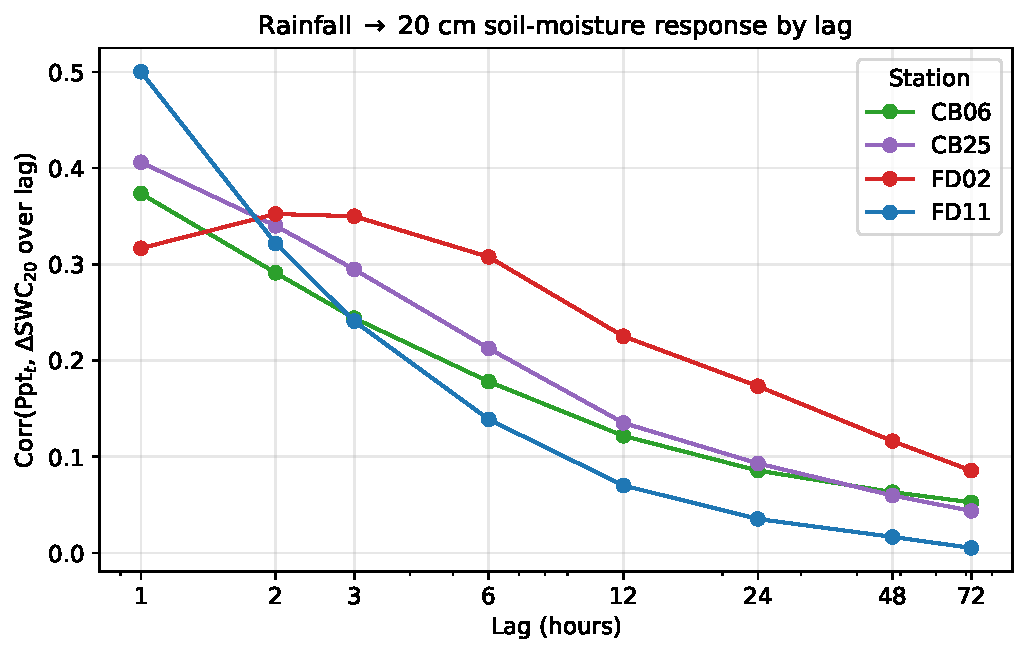
\includegraphics[width=0.72\textwidth]{fig_p1_lag_correlation.pdf}
\caption{Cumulative correlation between rainfall and 20\,cm soil-moisture change
versus lag, by station. The rainfall$\rightarrow$moisture response peaks at
1--2\,h and decays within a day.}
\label{fig:lag}
\end{figure}

\textbf{Depth.} Because rainfall wets shallow soil first, we repeat the analysis
at 5\,cm (Figure~\ref{fig:depth}). The depth effect is station-dependent: at the
driest station (FD02) rainfall couples far more tightly to 5\,cm ($r=0.56$) than
20\,cm ($r=0.33$), consistent with the expectation that near-surface moisture
responds more directly to rain. At FD11, however, the ordering reverses
($20\,\text{cm}=0.49 > 5\,\text{cm}=0.43$), and at CB06/CB25 the two depths are
comparable. So ``rain affects shallow soil more'' holds clearly only at the
driest site.

\begin{figure}[h]
\centering
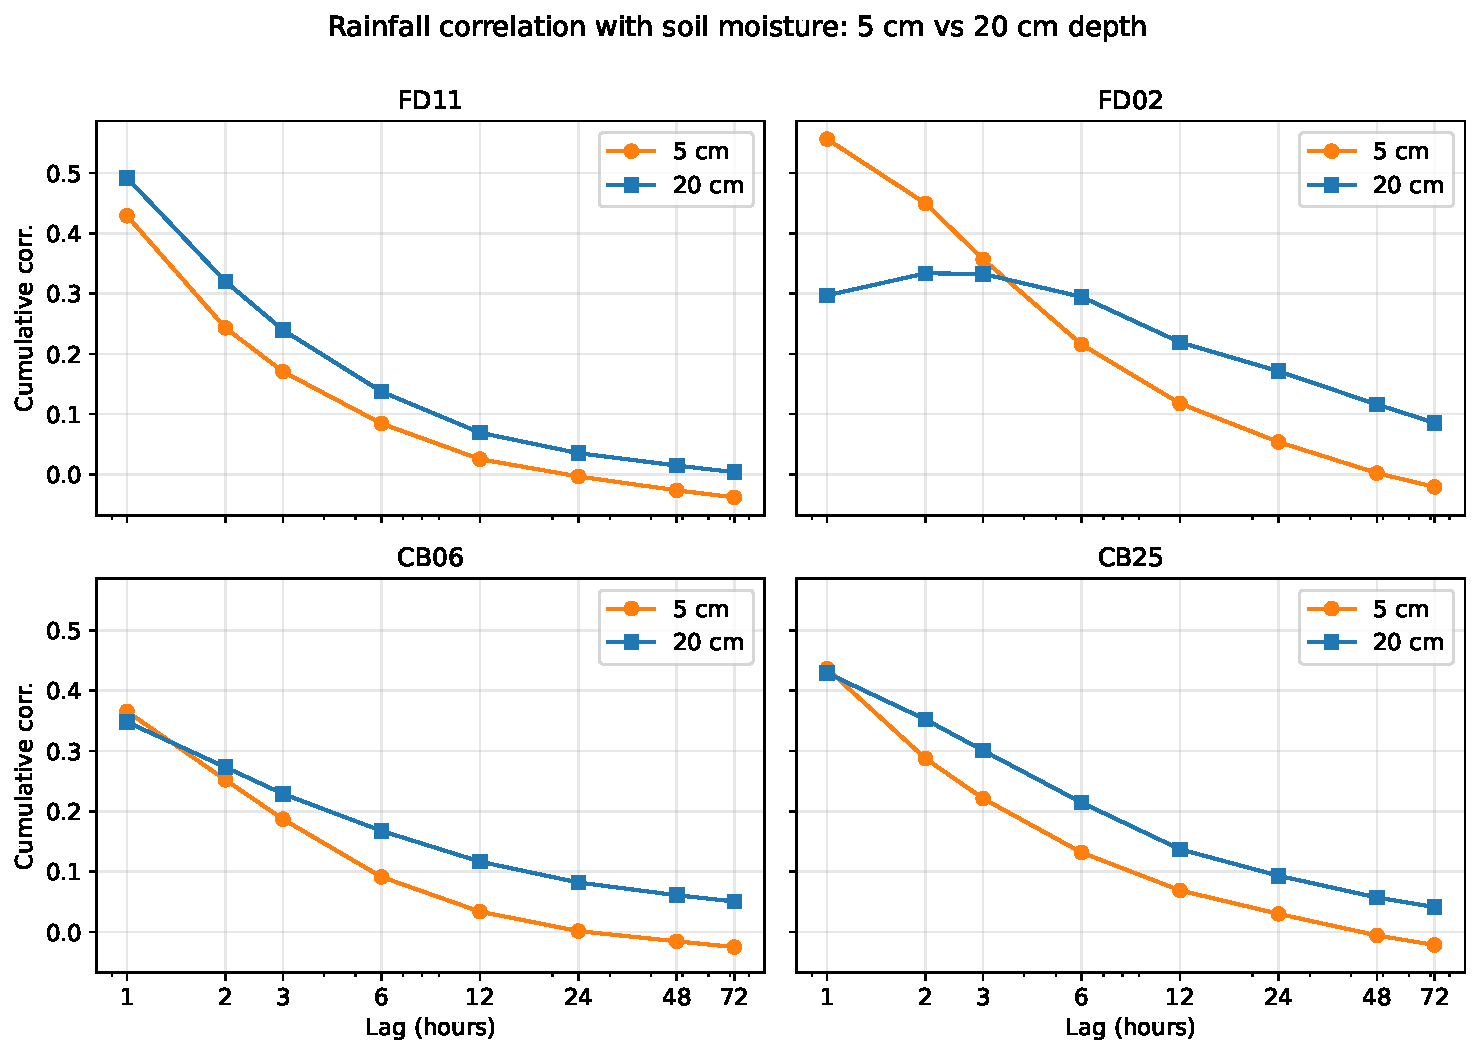
\includegraphics[width=0.85\textwidth]{fig_p4_lag_depth.pdf}
\caption{Rainfall correlation with soil moisture at 5\,cm vs 20\,cm. The 5\,cm
advantage is pronounced at FD02 but absent or reversed elsewhere.}
\label{fig:depth}
\end{figure}

\subsection{Forecast Error vs Horizon}

Table~\ref{tab:horizon} and Figure~\ref{fig:horizon} show that RMSE grows
monotonically with horizon and that the SWC-only CNN barely beats persistence.
Averaged over the five station-years, the CNN's improvement over persistence
shrinks from $+1.3\%$ at 24\,h to $-0.5\%$ at 168\,h. Soil moisture varies
slowly enough that the most recent observation is already a strong predictor, so
there is little headroom for a learned model on the RMSE metric.

\begin{table}[h]
\centering
\caption{Mean test RMSE (5 held-out station-years), SWC-only CNN vs persistence.
The improvement row is the mean of the five per-station-year percentage gains; it
differs slightly from the ratio of the rounded mean RMSEs above because stations
differ in RMSE scale.}
\label{tab:horizon}
\begin{tabular}{lccccc}
\toprule
\textbf{Model} & \textbf{H=24} & \textbf{H=48} & \textbf{H=72} & \textbf{H=96} & \textbf{H=168} \\
\midrule
Persistence    & 0.0139 & 0.0192 & 0.0230 & 0.0265 & 0.0349 \\
SWC-only CNN   & 0.0137 & 0.0190 & 0.0229 & 0.0263 & 0.0349 \\
\midrule
CNN impr.\ (\%) & $+1.3$ & $+0.8$ & $+0.3$ & $+0.3$ & $-0.5$ \\
\bottomrule
\end{tabular}
\end{table}

\begin{figure}[h]
\centering
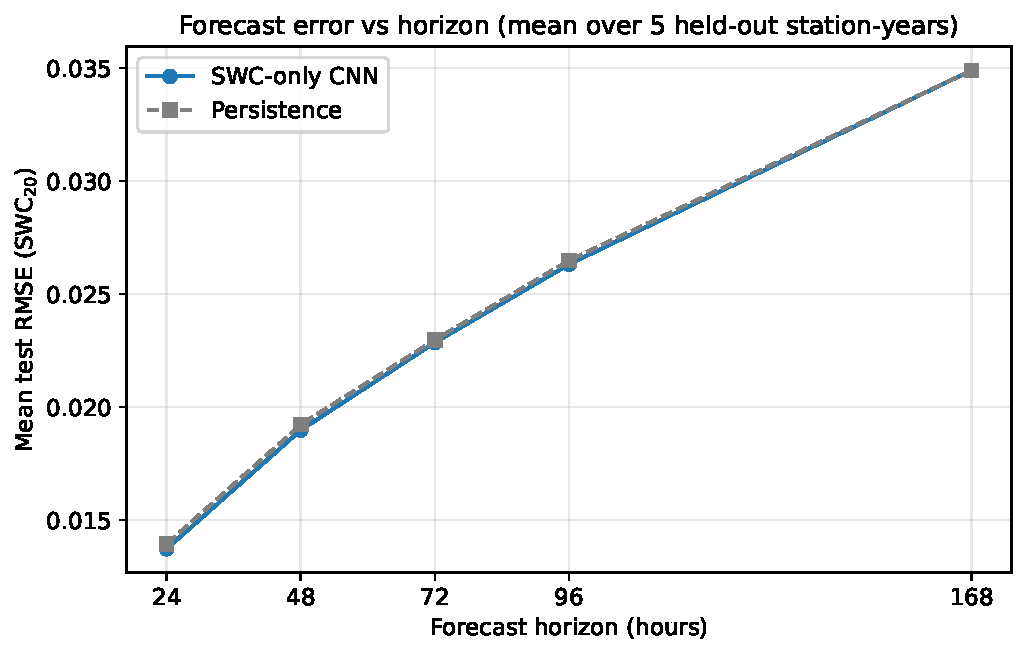
\includegraphics[width=0.7\textwidth]{fig_rmse_vs_horizon.pdf}
\caption{Mean RMSE versus forecast horizon; the SWC-only CNN tracks persistence
closely at all horizons.}
\label{fig:horizon}
\end{figure}

\subsection{Exogenous Feature Importance (Main Result)}

Table~\ref{tab:rank} ranks the five exogenous configurations by mean $\Delta\%$
over all 25 cells. \textbf{Every configuration has a negative mean}, and each
helps in only 8--10 of 25 cells. Adding air temperature (E) or single-step
rainfall (B) is least harmful on average ($-1.4\%$, $-1.5\%$); stacking many
features (F, combined met) is most harmful ($-3.9\%$), driven by large losses at
short horizons.

\begin{table}[h]
\centering
\caption{Exogenous feature comparison: mean \% RMSE change vs SWC-only over
25 station-year$\times$horizon cells (higher is better). Because every mean is
negative, this is a \emph{least-harm} ordering, not an importance ranking (see
text). ``$n$ better'' counts cells with improvement.}
\label{tab:rank}
\begin{tabular}{lcccc}
\toprule
\textbf{Configuration} & \textbf{Mean $\Delta\%$} & \textbf{$n$ better / 25}
& \textbf{Best cell} & \textbf{Worst cell} \\
\midrule
E: $+$ air temperature   & $-1.42$ & 8  & $+1.8$  & $-6.2$  \\
B: $+$ existing rain     & $-1.53$ & 8  & $+4.2$  & $-17.4$ \\
D: $+$ cumulative rain   & $-1.70$ & 8  & $+13.4$ & $-19.8$ \\
C: $+$ lagged rain       & $-2.91$ & 10 & $+3.0$  & $-24.1$ \\
F: combined met          & $-3.86$ & 9  & $+3.6$  & $-39.8$ \\
\bottomrule
\end{tabular}
\end{table}

The effect depends strongly on horizon and station
(Figure~\ref{fig:featheat}). At short horizons (24--48\,h) every exogenous
feature \emph{hurts} (combined met by $-11.7\%$ at 24\,h); only at 168\,h do
rainfall features turn marginally positive (cumulative rain $+1.7\%$, combined
met $+1.6\%$). By station, CB06 is harmed by every feature ($-3\%$ to $-13\%$),
whereas FD02---the driest, most rain-responsive station---benefits from
cumulative rainfall ($+6.2\%$ on average, up to $+13.4\%$ at 48\,h, its single
best result). This is the one place an exogenous feature delivers a clear,
repeatable gain, and it coincides with FD02's strong shallow-depth rain coupling
(Figure~\ref{fig:depth}).

\textbf{What ``importance'' can and cannot mean here.} Three distinct questions
must be separated. (i)~\emph{Which feature degrades RMSE least?}
Table~\ref{tab:rank} answers this---air temperature, then simple rainfall---but
because every mean is negative, it is an ordering of \emph{least harm}, not
evidence that any feature is beneficial. (ii)~\emph{Which feature helps at
particular stations?} Cumulative rainfall at FD02 is the only clearly positive,
repeatable case. (iii)~\emph{Which feature is genuinely important?} The present
design cannot answer this. Adding one group at a time on top of a bare
\texttt{SWC\_20} baseline confounds a feature's information content with the extra
estimation variance that any new input channel injects into a $\sim$2k-parameter
model on a strong-autoregressive target. We therefore \textbf{do not claim a
definitive exogenous-feature importance ranking}: since no configuration beats
SWC-only on average, the honest statement is that none of these exogenous features
is established as important for this CNN. Isolating a feature's \emph{marginal}
contribution would require a leave-one-group-out ablation from the full feature
set---removing one group at a time so the receptive field and channel count stay
comparable---together with multi-seed repetition to attach significance to any
differences (the between-cell standard deviations, 2--9\%, already exceed the mean
effects). We treat the per-feature means here as descriptive, not as a validated
ranking.

\begin{figure}[h]
\centering
\begin{subfigure}{0.56\textwidth}
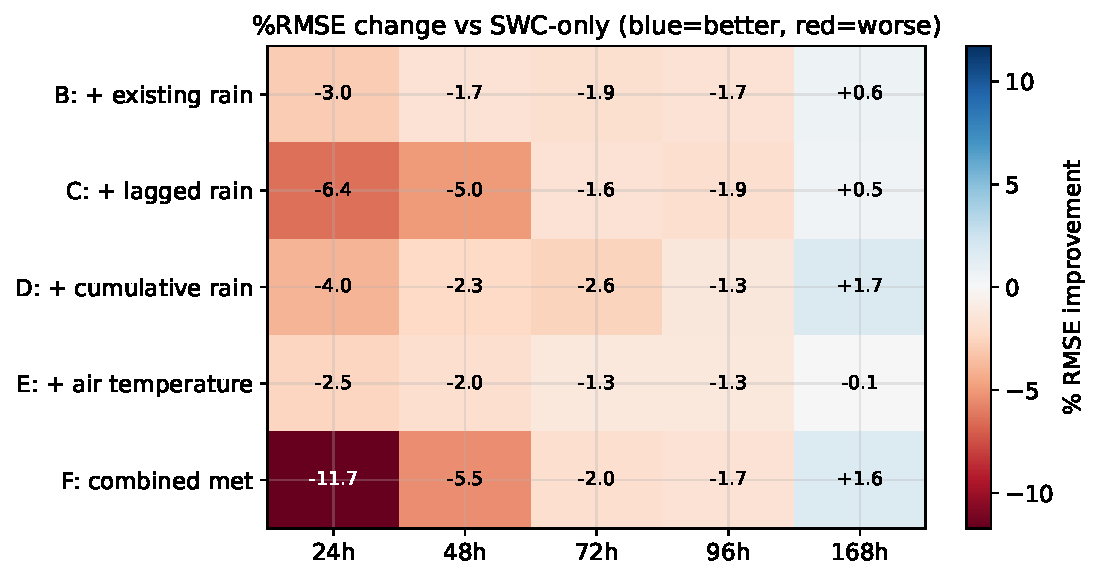
\includegraphics[width=\textwidth]{fig_feature_importance_heatmap.pdf}
\caption{By horizon}
\end{subfigure}
\begin{subfigure}{0.43\textwidth}
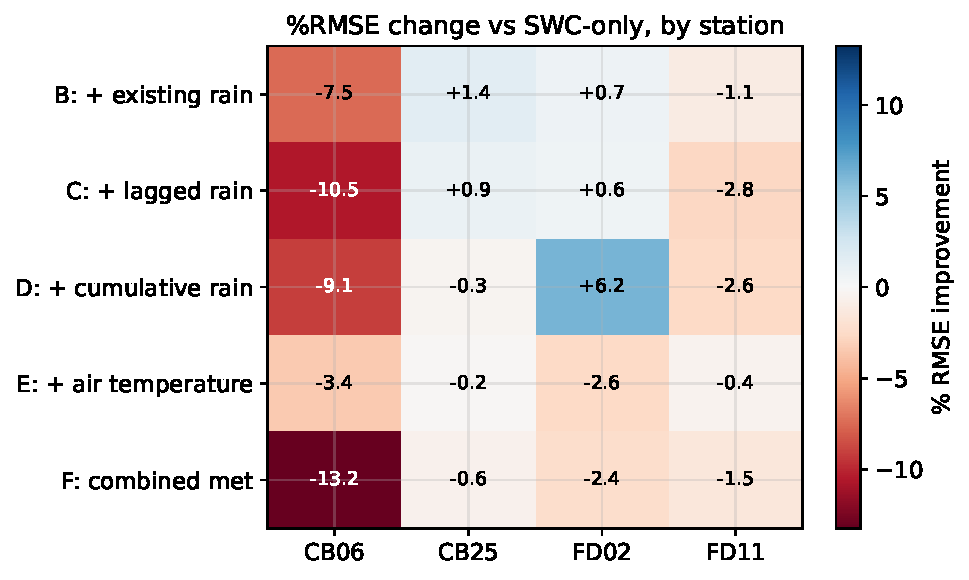
\includegraphics[width=\textwidth]{fig_feature_by_station.pdf}
\caption{By station}
\end{subfigure}
\caption{Mean \% RMSE change vs SWC-only. Blue = improvement, red = degradation.
Exogenous features hurt at short horizons and are neutral-to-slightly-positive
only at 168\,h; FD02 is the exception for cumulative rainfall.}
\label{fig:featheat}
\end{figure}

\subsection{CNN Hyperparameter Sweep}

A one-variable-at-a-time sweep at 72\,h on FD11--2023 (Table~\ref{tab:hp}) finds
the largest gains from a \emph{larger receptive field}: three convolutional
layers (RMSE 0.0265) or kernel size 7 (0.0266) improve on the two-layer, $K=3$
baseline (0.0279) by about 5\%. Wider filters alone help less, dropout hurts (the
model is already tiny), and lr $=10^{-3}$ is best. These gains were measured on a
single station-year and should not be assumed to generalize.

\begin{table}[h]
\centering
\caption{Hyperparameter sweep at H=72 on FD11--2023 (one variable changed at a
time). Lower RMSE is better.}
\label{tab:hp}
\begin{tabular}{lcccc}
\toprule
\textbf{Variant} & \textbf{Params} & \textbf{RMSE} & \textbf{Best epoch} \\
\midrule
layers = 3            & 7{,}905 & 0.0265 & 32 \\
kernel = 7            & 3{,}777 & 0.0266 & 17 \\
kernel = 5            & 2{,}721 & 0.0268 & 16 \\
filters = 32          & 6{,}401 & 0.0275 & 6  \\
baseline (k3, 2L, 16) & 1{,}665 & 0.0279 & 13 \\
dropout = 0.1         & 1{,}665 & 0.0288 & 2  \\
\bottomrule
\end{tabular}
\end{table}

\subsection{Training Diagnostics}

Per-epoch train/validation curves (Figure~\ref{fig:loss}) show healthy training:
validation loss reaches its minimum at a mean of epoch~12 of $\sim$20, and early
stopping restores those weights. Overfitting---measured as the rise in validation
loss from the best epoch to the final epoch---is mild overall (mean $+5.4\%$) but
grows with horizon, from $\sim$4.7\% at 24\,h to $+9.3\%$ at 168\,h, where the
mapping is hardest and the model is most tempted to fit training-set noise. This
confirms that validation-based early stopping is doing useful work, especially at
long horizons.

\begin{figure}[h]
\centering
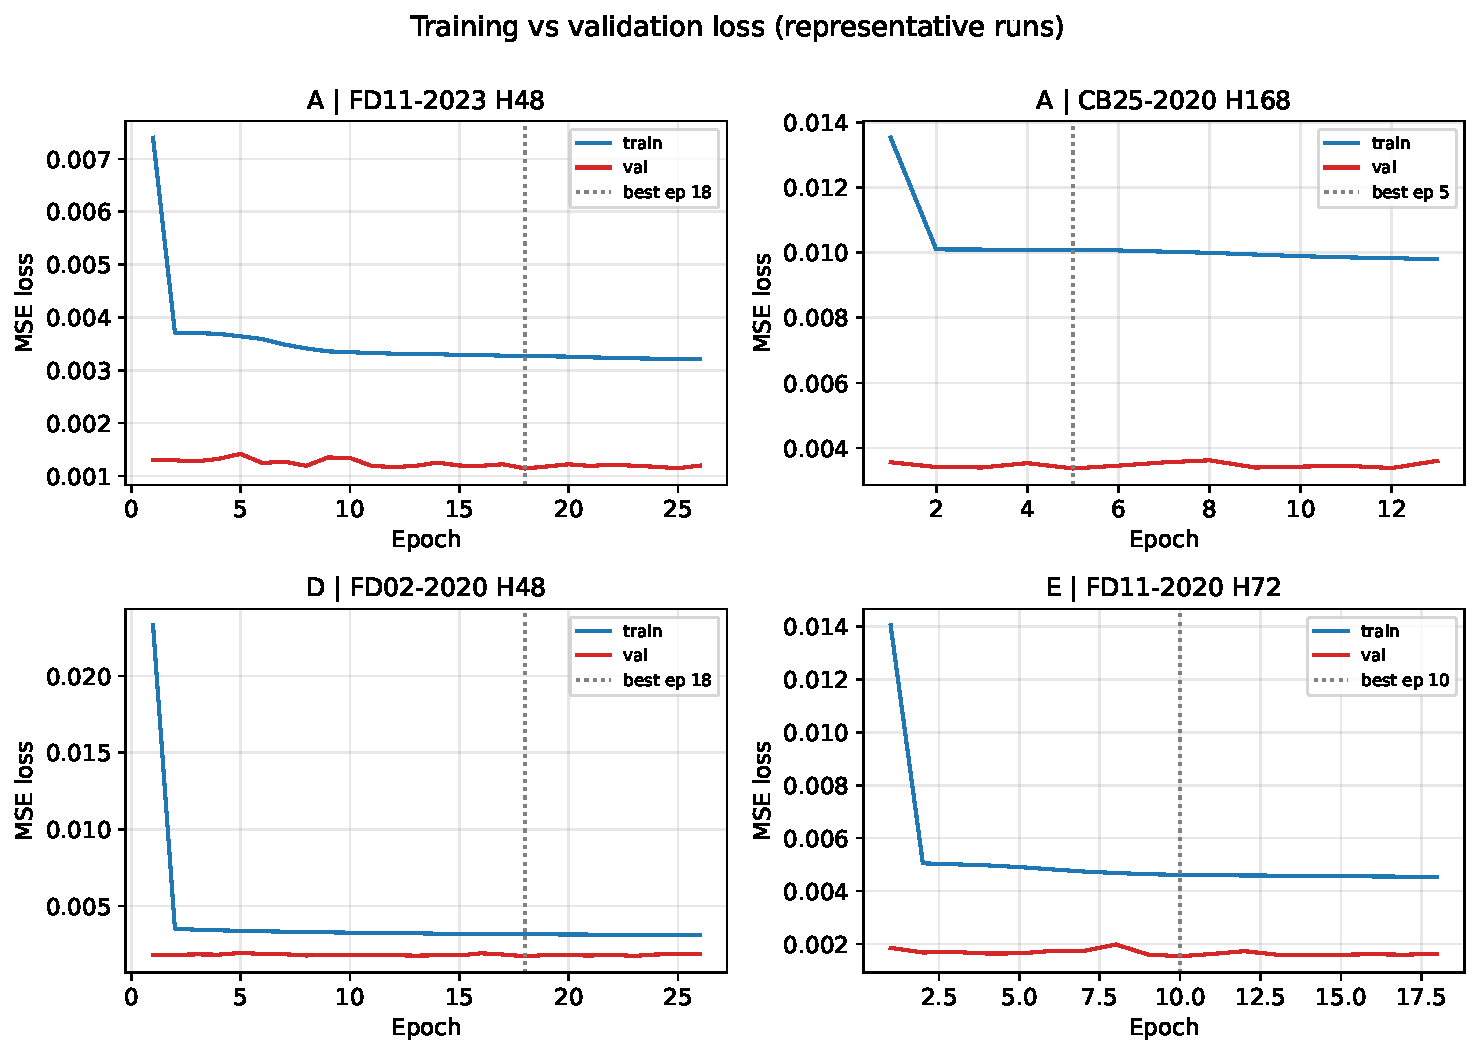
\includegraphics[width=0.85\textwidth]{fig_loss_curves.pdf}
\caption{Training vs validation MSE for representative runs; dotted line marks the
best-validation epoch restored by early stopping.}
\label{fig:loss}
\end{figure}

\subsection{Complementary Work: Classification and the Single-Station Study}

Two earlier lines of work provide qualitative context. A single-station study on
FD11 compared SmallCNN and LargerCNN against persistence and moving-average
baselines across window sizes and horizons, reaching the same horizon-dependent
conclusion as above: CNNs match persistence at short horizons and pull ahead only
near one week. A 12-class formulation (discretizing \texttt{SWC\_20} into
0.05-wide bins) compared three classification CNNs, of which a max-pooling variant
performed best, with errors almost always falling in an adjacent bin.
\emph{These two studies were carried out in the original exploratory notebook and
are not reproduced or re-verified in this repository; their detailed metrics are
therefore not restated here, and they are cited only as directionally consistent
context, not as results of the controlled experiments above.}

% ============================================================================
\section{Discussion}
% ============================================================================

\textbf{Historical soil moisture dominates.} The clearest message is that for
RMSE at these horizons, the target's own recent history carries nearly all the
predictive signal. The SWC-only CNN only marginally beats persistence, and adding
exogenous features more often hurts than helps. This is physically sensible:
20\,cm moisture changes slowly, so the last observation is an excellent short-term
predictor and leaves little for external drivers to add.

\textbf{When features help, and why.} The exceptions are informative. Exogenous
features are least harmful (and occasionally helpful) at the \emph{longest}
horizon, where the persistence signal has decayed and slow drivers such as
rainfall accumulation and temperature-driven drying matter more. The strongest
single benefit---cumulative rainfall at FD02---occurs at the driest, most
rain-responsive station, linking the forecasting result back to the lag analysis:
where rain explains more of the moisture dynamics, encoding it as a trailing
accumulation helps.

\textbf{Correlation is not predictive gain.} Lagged rainfall correlates with
soil-moisture change (Figure~\ref{fig:lag}), yet configuration~C (lagged rain)
is among the \emph{worst} performers. A feature can track the target's dynamics
and still fail to reduce forecast error once the target's own history is already
in the model, because the information is largely redundant and the extra input
dimensions add variance. This is a direct caution against reading the lag
correlations as evidence that lagged-rain features will improve the CNN.

\textbf{More features, more harm.} Combined met (F) is the worst configuration,
especially at short horizons. With a very small model and a strong autoregressive
signal, each additional input channel mostly adds noise and optimization
difficulty rather than signal.

% ============================================================================
\section{Limitations}
% ============================================================================

\begin{itemize}
    \item \textbf{Single seed.} All 150 runs use seed 42. Differences of a few
    percent between configurations are within plausible seed variance and should
    not be read as a confident ranking; multi-seed repetition is needed to
    separate signal from noise.
    \item \textbf{Architecture gains are local.} The $\sim$5\% improvement from a
    deeper/wider CNN was measured on one station-year (FD11--2023) at one horizon;
    it does not establish a general architectural improvement.
    \item \textbf{No leave-one-group-out ablation.} The feature evidence here is
    forward-selection (each group added to SWC-only). A complementary
    leave-one-out ablation from a combined model would strengthen the ranking;
    it was not available and is left as future work.
    \item \textbf{Coverage.} Four of 33 stations and five station-years were used.
    They span a useful wet/dry range but may not represent the full network.
    \item \textbf{Metric scope.} Conclusions are RMSE-centric. A feature that does
    not lower average RMSE might still improve tail behavior (e.g.\ rapid wetting
    events), which these aggregate metrics do not isolate.
\end{itemize}

% ============================================================================
\section{Conclusion}
% ============================================================================

On the TxSON data, with a shared 1D~CNN and a leakage-audited held-out
station-year protocol, \textbf{no exogenous feature consistently improves
20\,cm soil-moisture forecast RMSE over a soil-moisture-only model}. Historical
soil moisture is the dominant predictor at horizons from one day to one week.
Among external features, air temperature and simple rainfall are the least
harmful, while cumulative rainfall is the only feature with a clear, repeatable
benefit---and only at the driest, most rain-responsive station (FD02), mainly at
longer horizons. Rainfall correlates with soil-moisture change at a 1--2\,hour
lag and couples more to shallow soil at that station, but these correlations do
not translate into lower CNN error. Given the single-seed design, we present this
as evidence that the autoregressive signal dominates rather than as a definitive
feature ranking.

% ============================================================================
\section{Future Work}
% ============================================================================

\begin{enumerate}
    \item Repeat the strongest comparisons over multiple seeds to establish which
    differences are real.
    \item Add leave-one-feature-group-out ablations from a combined model to
    corroborate the forward-selection ranking.
    \item Forecast shallow moisture (\texttt{SWC\_5}) directly, where rainfall
    coupling is stronger, and test whether exogenous rainfall features help more.
    \item Evaluate event-focused metrics (performance during rapid wetting) in
    addition to aggregate RMSE.
    \item Extend to more TxSON stations and compare against an LSTM baseline under
    the identical pipeline.
\end{enumerate}

\bibliographystyle{plain}
\bibliography{references}

\end{document}
